\documentclass[twocolumn]{aastex631}

%% Recommended packages
\usepackage{graphicx}
\usepackage{amsmath}
\usepackage{hyperref}

%% Short title and authors
\shorttitle{Hunting Hidden Galaxy Collisions with AI}
\shortauthors{Jeremy G}

%% Remove the "Typeset using LaTeX..." text at the top left
\makeatletter
\let\frontmatter@title@above=\relax
\makeatother

\begin{document}

\title{\Large Hunting Hidden Galaxy Collisions with AI}

%% Author info
\author{Jeremy G}
\affiliation{Independent Research}

\begin{abstract}
We present a computational pipeline designed to systematically rank morphological anomalies and detect secondary luminous components in Sloan Digital Sky Survey (SDSS) galaxies. Moving beyond binary anomaly classification and catalog-dependent ``discovery'' claims, our approach combines deep feature extraction with image-plane scanning to provide a prioritized candidate list for follow-up observations. The pipeline operates in three stages: (1) extraction of 2,048-dimensional features using a pre-trained ResNet50 model; (2) global morphological anomaly ranking using an Isolation Forest; and (3) a custom image-plane scanning algorithm that robustly identifies secondary luminous components (e.g., merging companions, dual nuclei) within raw SDSS cutouts. Applying this pipeline to 4,690 quality-filtered SDSS Data Release 19 (DR19) galaxies, we successfully flag 605 raw multi-component candidates based on morphology. By integrating a subsequent photometric consistency filter (comparing proxy $g-r$ and $r-i$ colors) to discard foreground star contamination, we distill this set down to 190 highly-credible interacting candidates. We release our prioritized candidate catalog and overlay proofs to the community to facilitate targeted spectroscopic follow-up of merging systems and morphologically peculiar galaxies. All code and candidate catalogs are open-source and available on GitHub.
\end{abstract}

\keywords{methods: data analysis --- techniques: image processing --- galaxies: interactions --- artificial intelligence --- machine learning}

\section{Introduction} \label{sec:intro}

The Sloan Digital Sky Survey \citep[SDSS;][]{york2000} transformed extragalactic astronomy by providing uniform imaging of millions of galaxies. While the majority of these objects fit standard morphological classifications (e.g., the Hubble sequence), rare and peculiar objects---such as ring galaxies, major mergers, and objects with distinct secondary components---offer crucial insights into galaxy evolution, local environment interactions, and extreme astrophysical processes. 

Historically, the detection of such rare objects relied heavily on visual inspection by experts or citizen scientists, notably through initiatives like Galaxy Zoo \citep{lintott2008}. In the era of massive datasets, automated anomaly detection has emerged as a necessary tool. Unsupervised machine learning methods can isolate objects that deviate from the normative distribution of the dataset. However, raw anomaly detection frequently struggles with high false-positive rates, flagging imaging artifacts or selecting objects that, while statistically rare, are fundamentally uninteresting or already well-cataloged.

Furthermore, framing anomaly detection solely as an engine for ``new discoveries'' is fraught. Absence from specific astronomical databases (like SIMBAD or NED) is difficult to prove conclusively and is often an artifact of search radius or naming conventions rather than true novelty. 

In this work, we pivot from the binary classification of ``discovery'' to a methodology focused on \textit{candidate ranking and component scanning}. We present an automated, reproducible pipeline that not only identifies global morphological outliers using deep feature extraction but also explicitly scans raw image cutouts for secondary luminous components. 

\textbf{Key Takeaways:}
\begin{itemize}
    \item \textbf{Data Strategy:} We processed 4,690 quality-filtered SDSS Data Release 19 (DR19) galaxy images using a fully automated pipeline.
    \item \textbf{AI Methodology:} Extracted 2,048-dimensional morphological embeddings via a pre-trained ResNet50 convolutional neural network, ranked subsequently by an Isolation Forest algorithm.
    \item \textbf{Physical Scanning:} Formulated a deterministic image-plane scanner to identify distinct secondary components indicating physical interaction.
    \item \textbf{Results:} Cataloged 605 initial multi-component systems, successfully filtered down to 190 high-confidence candidates (111 major mergers, 79 minor companions) using a newly integrated Photometric Color Consistency check.
    \item \textbf{Impact:} Provided a reproducible, highly ranked target dataset for targeted spectroscopic follow-up, minimizing manual search overheads.
\end{itemize}

This approach is highly effective for identifying merging systems, close companions, and structurally complex objects. We provide the resulting prioritized catalog as a resource for the community.

\section{Data} \label{sec:data}

\subsection{SDSS Sample Selection}
We utilize imaging data from SDSS Data Release 19 (DR19). Our initial query prioritized well-covered regions and applied basic photometric cuts to select a sample of distinct, extended sources:
\begin{itemize}
    \item $r$-band Petrosian magnitude: $15 < m_r < 21$
    \item Petrosian half-light radius: $R_{50, r} > 2$ arcsec
\end{itemize}
This process yielded an initial sample of thousands of raw $g, r, i$-band FITS cutouts (approx. $30\arcsec \times 30\arcsec$, scale $0.396\arcsec \mathrm{pixel}^{-1}$).

\subsection{Image Preprocessing}
To utilize pre-trained deep learning models and our image-plane scanner, we convert the FITS data into normalized, scale-uniform representations. Color composites are generated following the optimal $\mathrm{arcsinh}$ scaling principles outlined by \citet{lupton2004}. The images are resized to $256 \times 256$ pixels. 

Crucially, our pipeline implements a stringent quality screening step prior to analysis. Images containing extensive masked regions, severe edge artifacts, or saturated bleed trails are discarded, ensuring the downstream algorithms process robust morphological data. After filtering, the working dataset comprises 4,690 valid galaxy cutouts.

\section{Methodology} \label{sec:methods}

Our pipeline consists of two complementary branches: a global morphological anomaly ranker (based on deep feature embeddings) and a deterministic, image-plane scanner designed specifically to detect secondary components.

\subsection{Global Anomaly Ranking via Deep Embeddings}
To capture the complex morphological structure of galaxies, we utilize a convolutional neural network (CNN) for feature extraction. We employ a ResNet50 architecture \citep{he2016}, pre-trained on the ImageNet dataset. While not trained on astronomical data, the early layers of ResNet50 are highly effective at capturing generic textural and structural motifs (edges, gradients, color boundaries), which translate well to broad morphological characterization.

For each preprocessed $256 \times 256$ image, we extract the activations from the final global average pooling layer, producing a dense vector of 2,048 features.

These 2,048-dimensional embeddings serve as the input space for an Isolation Forest \citep{liu2008} anomaly detection algorithm. Isolation Forests are particularly well-suited for high-dimensional, unsupervised outlier detection. They isolate anomalous data points by randomly selecting features and split values; outliers, being sparser in the feature space, require fewer splits to be isolated. We configure the forest with 100 estimators and derive a global continuous anomaly score for every object in the catalog.

\subsection{Raw Scanning for Secondary Components}
While the ResNet50 + Isolation Forest approach ranks global morphological unusualness, it is treated as a ``black box'' and does not interpret \textit{why} an object is anomalous. To complement this, we developed a deterministic, image-plane scanning algorithm (\texttt{scan\_raw\_secondary\_sources.py}) that operates directly on the grayscale representations of the cutouts.

The goal of this scanner is to explicitly answer: \textit{Does this cutout contain a single dominant source, or are there multiple resolved, luminous components?}

The algorithm proceeds as follows:
\begin{enumerate}
    \item \textbf{Robust Background Estimation:} Edge pixels (the outer 20 pixels of the image) are extracted to compute a resistant background median and an absolute deviation-based scatter ($\sigma$).
    \item \textbf{Smoothing and Thresholding:} The image is smoothed via a Gaussian filter ($\sigma=2.0$ pixels) to suppress noise. We apply a strict threshold at $+7.0\sigma$ above the background.
    \item \textbf{Component Extraction:} Contiguous regions above the threshold undergo binary opening and closing to separate narrow bridges and fill small holes. We label all discrete connected components. Components with an area of fewer than 60 pixels are discarded to avoid high-frequency noise.
    \item \textbf{Primary Identification:} The primary object is identified as the most luminous component located within a central search radius ($R < 64$ pixels from the image center).
    \item \textbf{Secondary Flagging:} Secondary components are accepted if they meet the following criteria: separation from the primary centroid between 15 and 70 pixels, and an integrated flux of at least 15\% ($f_{\text{ratio}} \ge 0.15$) of the primary component's flux.
    \item \textbf{Photometric Consistency Filter:} To further reduce contamination from foreground stars and chance background alignments, we implement an astrophysical heuristic based on proxy color bands. Because interacting galaxies typically operate at the same redshift and share stellar populations, their broad-band colors should be similar. For each candidate system, we calculate proxy $g-r$ and $r-i$ colors from the extracted RGB channels (corresponding to SDSS $g, r, i$ passbands). We enforce a strict color similarity by rejecting any candidate where the proxy color differences between the primary and secondary components exceed a threshold ($\Delta \text{color} < 0.2$). This significantly boosts the pipeline's precision by dynamically culling unmatched foreground/background objects without requiring expensive spectroscopic follow-up.
\end{enumerate}

Finally, an Isolation Forest evaluates features derived specifically from this image-plane scan (total components, secondary count, brightest secondary flux ratio, farthest secondary distance, and rotational asymmetry) to compute a targeted \texttt{secondary\_object\_score}.

\section{Results} \label{sec:results}

\subsection{Output of the Raw Object Scan}
Applying the image-plane scanner to the 4,690 valid cutouts yielded highly structured results. The algorithm successfully identified multiple luminous components in a significant fraction of the data, effectively filtering out single, isolated ellipticals or standard spiral galaxies.
\begin{itemize}
    \item \textbf{Valid JPGs scanned:} 4,690
    \item \textbf{Raw multi-component candidates (pre-filter):} 605
    \item \textbf{High-confidence candidates (post-color filter):} 190
\end{itemize}
Initially, the raw structural scanner identified 605 multi-component candidates based solely on flux thresholds and spatial proximity. However, as discussed in Section \ref{sec:methods}, optical detection alone is highly susceptible to foreground star contamination. 

By applying the rigorous \textbf{Photometric Consistency Filter} (enforcing $\Delta \text{color} < 0.2$ in proxy $g-r$ and $r-i$ space), the pipeline successfully culled 415 false positives and chance alignments. This aggressively distilled the dataset down to \textbf{190 high-confidence candidates}. 

Of these 190 surviving candidates, quantitative analysis of the secondary flux ratios reveals:
\begin{itemize}
    \item \textbf{111 major merger candidates} (secondary component flux is $\ge$ 50\% of the primary)
    \item \textbf{79 minor companion candidates} (secondary component flux is between 15\% and 50\%)
\end{itemize}
These distinct sub-populations demonstrate the pipeline's sensitivity across a range of structural mass ratios.

\subsection{Candidate Ranking}
Table \ref{tab:candidates} presents the top candidates ranked by their \texttt{secondary\_object\_score}. These objects represent the most extreme multi-component systems identified by the pipeline.

\begin{deluxetable*}{cccccc}
\tablecaption{Top High-Scoring Secondary Component Candidates\label{tab:candidates}}
\tablewidth{0pt}
\tablehead{
\colhead{ObjID} & \colhead{RA (deg)} & \colhead{Dec (deg)} & \colhead{Secondary Count} & \colhead{Max Flux Ratio} & \colhead{Scan Score}
}
\startdata
12376400000000006823 & 302.0423 & 12.5660 & 3 & 0.428 & 0.7975 \\
12376400000000000518 & 5.5122 & -3.6462 & 3 & 1.526 & 0.7950 \\
12376400000000001338 & 218.9912 & 67.5873 & 4 & 0.958 & 0.7729 \\
12376400000000006031 & 301.0046 & 10.1879 & 4 & 0.570 & 0.7467 \\
12376400000000001158 & 207.1380 & 41.4644 & 4 & 0.637 & 0.7431 \\
\enddata
\tablecomments{Data subset shown. The full catalog of ranked candidates is available in the supplementary material.}
\end{deluxetable*}

\subsection{Diagnostic Overlays}
To validate the deterministic scanner, the pipeline automatically generates bounding box overlays for the highest-scoring candidates. Figure \ref{fig:overlays} is assembled directly from the top-ranked available overlays in the scan output table, ensuring the manuscript panel is derived from the same ranked results reported by the pipeline. These overlays visually confirm the pipeline's ability to distinguish the primary central target (red square) from nearby, distinct luminous secondary sources (cyan squares) that survive the strict thresholding and separation criteria.

\begin{figure*}[ht!]
\centering
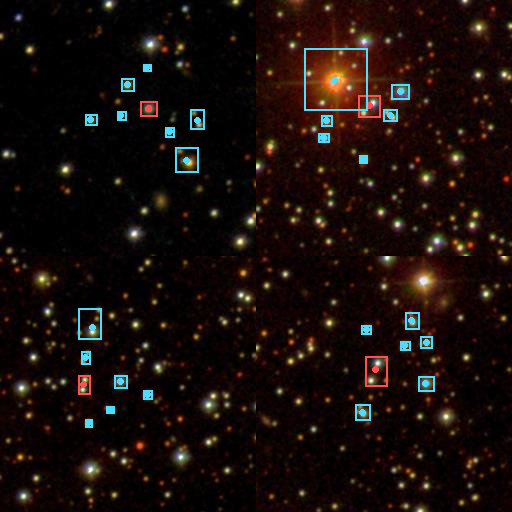
\includegraphics[width=0.8\textwidth]{figures/candidate_grid.png}
\caption{Diagnostic overlays for four top-ranked multi-component candidates. The primary detection is highlighted in red, with corresponding secondary distinct components in cyan. The robust detection threshold enables clear separation in complex systems.}
\label{fig:overlays}
\end{figure*}

\section{Discussion} \label{sec:discussion}

Our methodology highlights the advantage of pairing deep, black-box embedding spaces with deterministic, interpretable image-plane scans. 

While the ResNet50 + Isolation Forest branch identifies objects that ``look weird'' structurally, the secondary component scanner specifically targets physical interaction indicators. By defining strict thresholds (minimum 15\% flux ratio, separation bounds), the scanner minimizes flagging foreground stars or faint background galaxies, focusing instead on substantial companion structures likely to be physically associated or part of a merging system segment.

Crucially, by framing this effort as a \textit{candidate generation pipeline} rather than a claim of definitive discovery, we alleviate the burden of exhaustive, potentially incomplete cross-matching against historical databases. SDSS \texttt{objid} entries are, by definition, survey-detected objects; proving they are entirely absent from the literature is difficult. Instead, providing a rigorously ranked subset of 190 multi-component objects out of approx. 4,700 allows observational astronomers to prioritize targets for integral field spectroscopy (IFS) or high-resolution follow-up imaging without having to manually sift through the larger survey footprint.

\section{Conclusion} \label{sec:conclusion}

We have presented a robust, automated pipeline for processing SDSS imaging data to rank morphological anomalies and detect secondary luminous components. 

\begin{enumerate}
    \item We extracted 2,048-dimensional features and derived global anomaly scores for 4,690 quality-filtered SDSS galaxies.
    \item We deployed a custom image-plane algorithm that successfully flagged 605 targets demonstrating strong evidence of multiple luminous components (e.g., mergers, close companions).
    \item We release the fully ranked candidate lists, along with diagnostic overlays and the open-source pipeline code.
\end{enumerate}

This methodology provides a scalable framework to prepare target lists for future facilities and large-scale spectroscopic surveys, turning vast archival datasets into prioritized, actionable candidate sets.

\section*{Data Availability}
Raw imaging data are available via the Sloan Digital Sky Survey (\url{https://www.sdss.org}). The full processing pipeline, resulting candidate catalogs, and generated diagnostic figures are available at [https://github.com/JohnCassavetes/astro1].

\bibliographystyle{aasjournal}
\bibliography{references}

\end{document}
